%\let\oldthesubsection=\thesubsection
\renewcommand{\thesubsection}{\Roman{subsection}}

%A dolgozat olyan nyelvtechnológiai előfeldolgozó algoritmusokat mutat be, melyek hatékonyan képesek szövegek elemzésére agglutináló nyelvek esetén. 
%Vizsgálataimat magyar nyelvre végeztem, de a módszerek kidolgozása során törekedtem a nyelvfüggetlenségre. 
%Így, a bemutatott eljárások más, hasonló struktúrájú nyelvek esetén is sikerrel alkalmazhatóak.
%%Munkám során kiemelt szerep jutott a morfológiai egyértelműsítés feladatának, mivel ennek kimenetére számtalan információkinyerő rendszer épít.
%
%Az első téziscsoportban a általános magyar nyelvű morfológiai egyértelműsítés területén elért eredményeimről számolok be. 
%Ezt követően bemutatom a létrehozott annotáló eszköz egy gyakorlati alkalmazását. 
%Végül, ismertetem azon új előfeldolgozó eljárásokat, melyek zajos (klinikai) szövegeket is hatékonyan képesek elemezni.
%

\subsection{Effective morphological tagging methods for morphologically rich languages} %TODO: igeidők
\label{thes:morf}

Full morphological tagging is a complex task composed of two parts. 
Beside identifying morpho-syntactic tags, lemmata of words must be computed as well.
While the first task is a well-known problem of \acrlong{nlp}, the latter one is often neglected.
Results are summarized by describing  the new lemmatization method first, followed by the full tagging systems. 


\begin{core}
\begin{thesis}\label{thes:morf-lemma}
I developed a new lemmatization method for agglutinative languages.
The presented algorithm is based on the output of a morphological analyzer. It can handle both known and unknown words effectively by incorporating diverse stochastic models. 
Results presented show that the new system has high accuracy on Hungarian texts.
\end{thesis} 

\begin{pub}
\cite{Orosz2011,Orosz2012,Orosz2012a,Orosz2013a}
\end{pub}
\end{core}

The proposed algorithm performs lemmatization in two steps. 
First, it uses a morphological analyzer and a guesser component to generate lemma candidates, then disambiguation is performed using stochastic models.
The latter part is carried out calculating the score ($S$) of each lemma ($l$) for a given word ($w$) and tag ($t$) using the interpolation of two different models:
\begin{equation} %\label{lemma-interpolated}
S(l|w,t) = P(l)^{\lambda_1} P(l,t|w)^{\lambda_2}
\end{equation}

The system combines a simple unigram model with the output of a suffix-based guesser. 
To calculate the lambda parameters, guesses of models are evaluated on the training data, then the better model's score gets increased while that of the worse one is decreased.

Several experiments have been presented on the Szeged Corpus showing that the proposed method has superior accuracy for Hungarian compared to other available tools. 

\thesisline%%%%%%%%%%%%%%%%%%%%%%%%%%%%%%%%%%%%%%%%%%%%%%%%%%%%%%%%%%%%%%%%%%%


\begin{core}
\begin{thesis}\label{thes:morf-tagging}
I designed a hybrid morphological tagging system (PurePos\footnote{The presented system is open source and is freely available at \href{https://github.com/ppke-nlpg/purepos}{https://github.com/ppke-nlpg/purepos}}) for less-resourced and agglutinative languages.
The method relies on stochastic methods incorporating the output of a morphological analyzer.
Its lemmatization component utilizes algorithms presented in Thesis \ref{thes:morf-lemma}.
Furthermore, the tool is built up in a way to be able to incorporate domain-specific rules effectively.
Experiments confirm its state-of-the-art accuracy for Hungarian.
\end{thesis}

\begin{pub}
\cite{Orosz2011,Orosz2012,Orosz2012a,Orosz2013a}
\end{pub}
\end{core}

\begin{figure}[ht] 
  \centering
  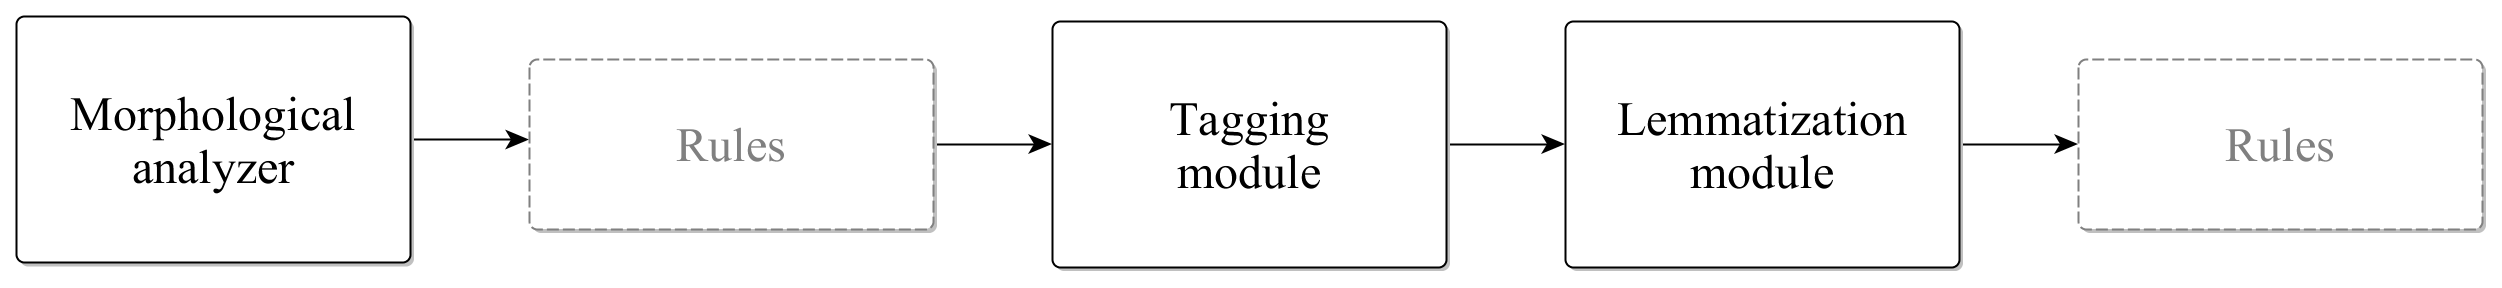
\includegraphics[width=1\textwidth]{MorphTagging/architecture.png} 
  \caption{The architecture of the full morphological tagging tool}
  \label{fig:purepos-arch_en}
\end{figure}

The architecture of PurePos (cf. Figure \ref{fig:purepos-arch_en}) is built up to allow multiple models cooperating effectively. 
The disambiguation is carried out in multiple steps.
The data flow starts from a \acrshort{ma} providing word analyses as \emph{(lemma, tag)} pairs. 
Next, trigram-tagging methods (see \cite{Brants2000,Halacsy2007}) are employed for selecting morpho-syntactic labels of words. 
%In fact, these algorithms have been adapted to fit agglutinative languages.
Finally, lemmatization is carried out employing the methods presented in Thesis \ref{thes:morf-lemma}. 

\begin{figure}[H]
  \centering
  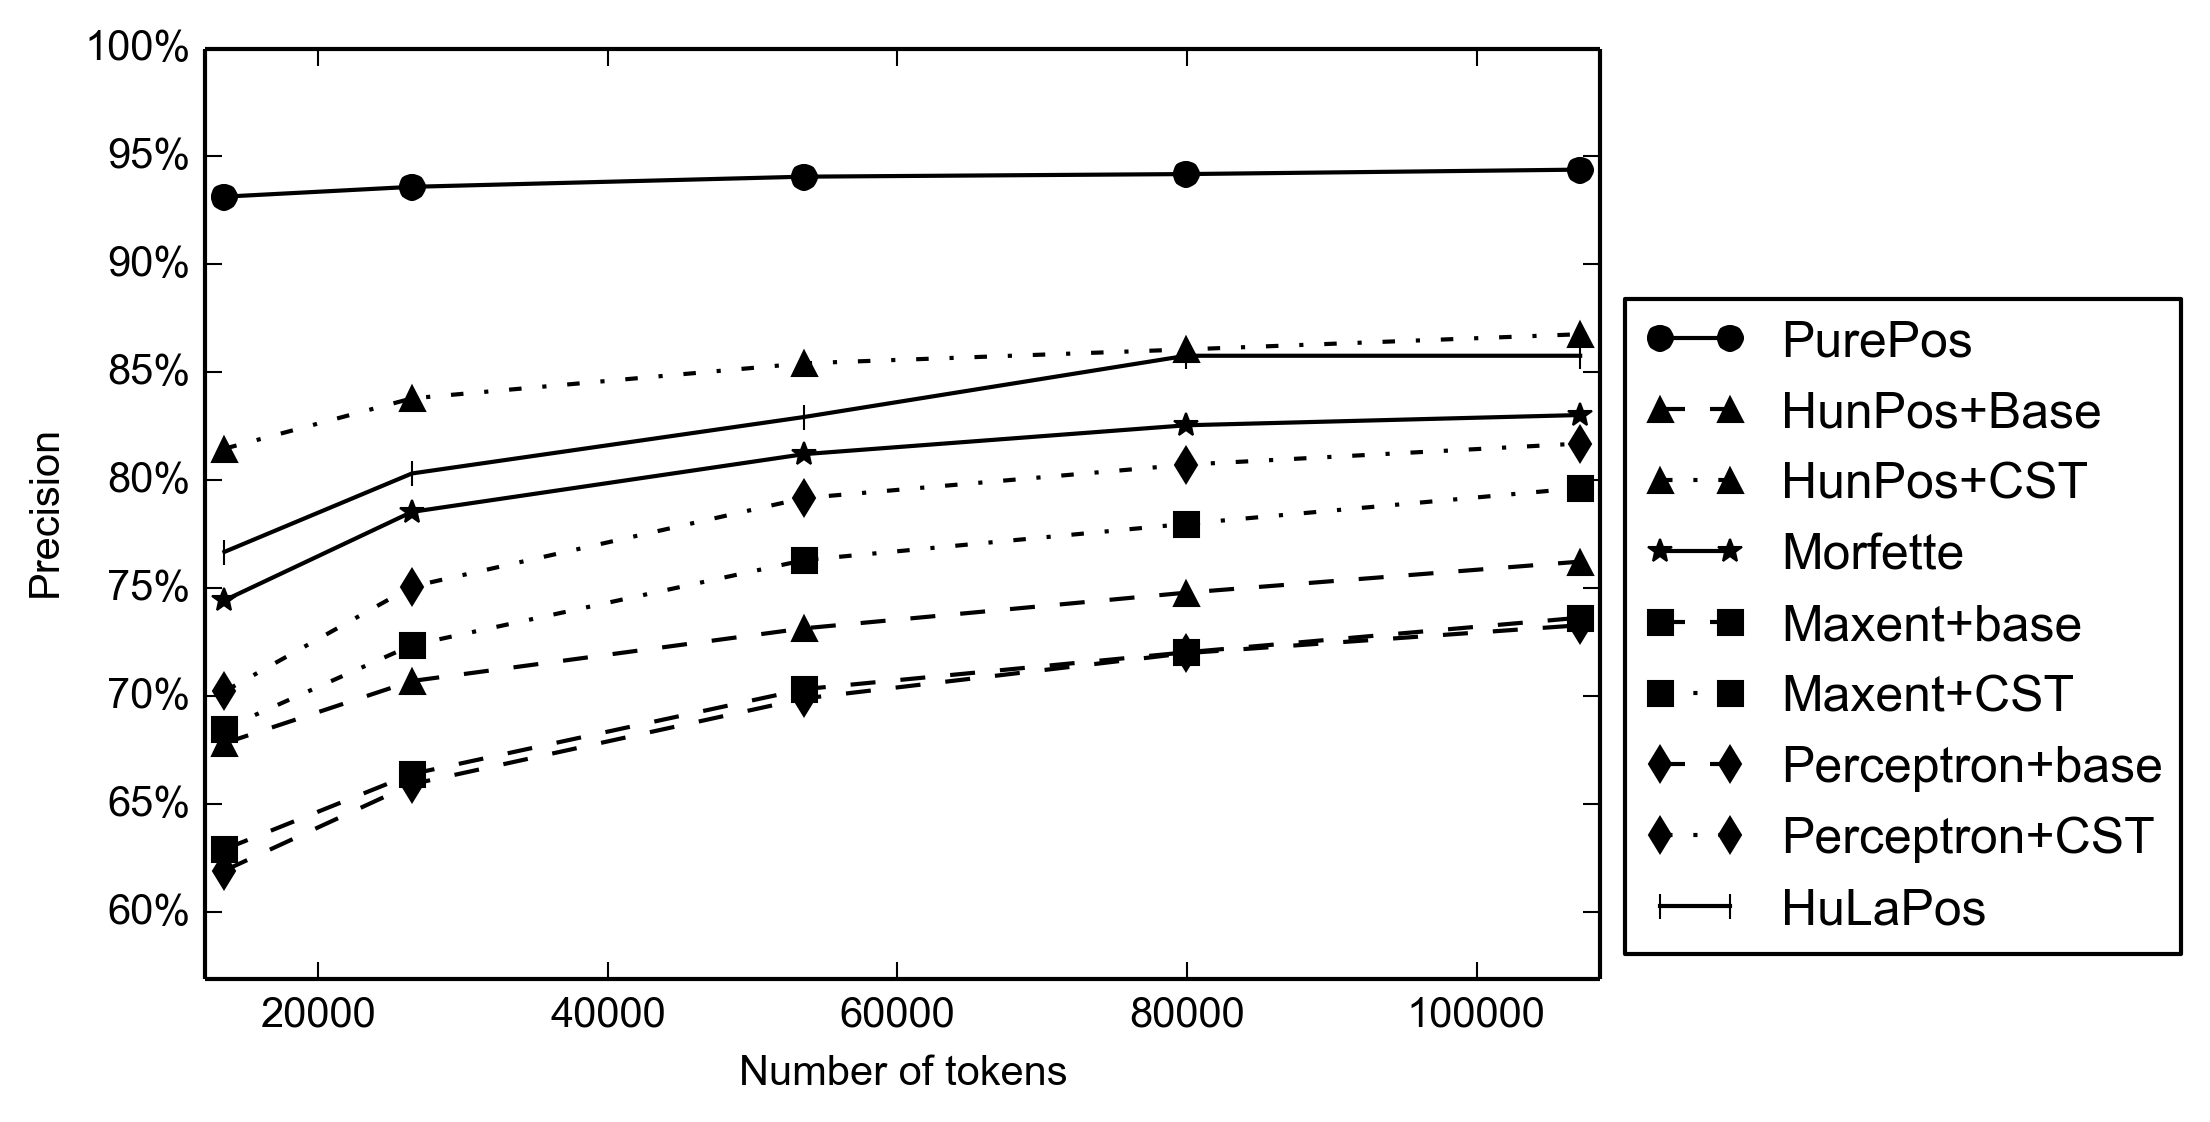
\includegraphics[width=1\textwidth]{MorphTagging/msd_token.png}
  \caption{Learning curves of full morphological taggers on the Szeged Corpus (using Humor labels)}
  \label{fig:humor-token_en}
\end{figure}

Several experiments were carried out measuring the performance of PurePos on the Szeged Corpus \cite{Csendes2004}.
Results show that the new method yields 96.26\% full tagging accuracy, which is the highest one amongst available tools.
Moving on, I also compared existing tagging systems with the presented one on a less-resourced scenario.
These experiments showed (cf. Figure \ref{fig:humor-token_en}) that PurePos can be successfully used even when the training dataset is limited.
Finally, all the hybrid enhancements of PurePos ware evaluated one-by-one, showing that they can be used to fix several sorts of errors.


\thesisline%%%%%%%%%%%%%%%%%%%%%%%%%%%%%%%%%%%%%%%%%%%%%%%%%%%%%%%%%%%%%%%%%%%%%

Although, methods of Thesis group \ref{thes:morf-tagging} have high accuracy, it was shown that they can be improved further.  
Therefore, a combination technique is presented increasing the ceiling of morphological tagging tools' performance for agglutinative languages.


\begin{core}
\begin{thesis}
I developed a methodology for combining morphological tagging systems effectively.
The system presented selects the best lemma and tag candidates separately using two different combination methods.
These components are trained with cross-validation using instance based learning.
I showed that my method can significantly reduce the number of errors of existing annotation tools.
\end{thesis}

\begin{pub}
\cite{Laki2013a,Orosz2013c,Orosz2013d} 
\end{pub}
\end{core}

First of all, the discrepancy of tagging systems was investigated. 
For this, I designed a new metric (Own Error Rate) which measures the differences of output of taggers.
It turned out that the most typical mistakes of HuLaPos \cite{Laki2013} and PurePos are different enough to be aggregated.

Following this, the most common combination techniques were investigated considering their applicability to full morphological tagging.
Next, a new combination method was presented involving adapted feature sets for morphologically rich languages.
It utilizes instance based learning \cite{Aha1991} and trains classifiers with cross-validation, which
can employ the whole training dataset for both the baseline tools and the level-one learners. %TODO Nóri fordítás
The novelty of the presented method is its architecture (cf. Figure \ref{fig:comb3_en}) allowing us to utilize different combiners for the lemmatization and \acrshort{pos} tagging subtasks.

\begin{figure}[H]
  \centering
  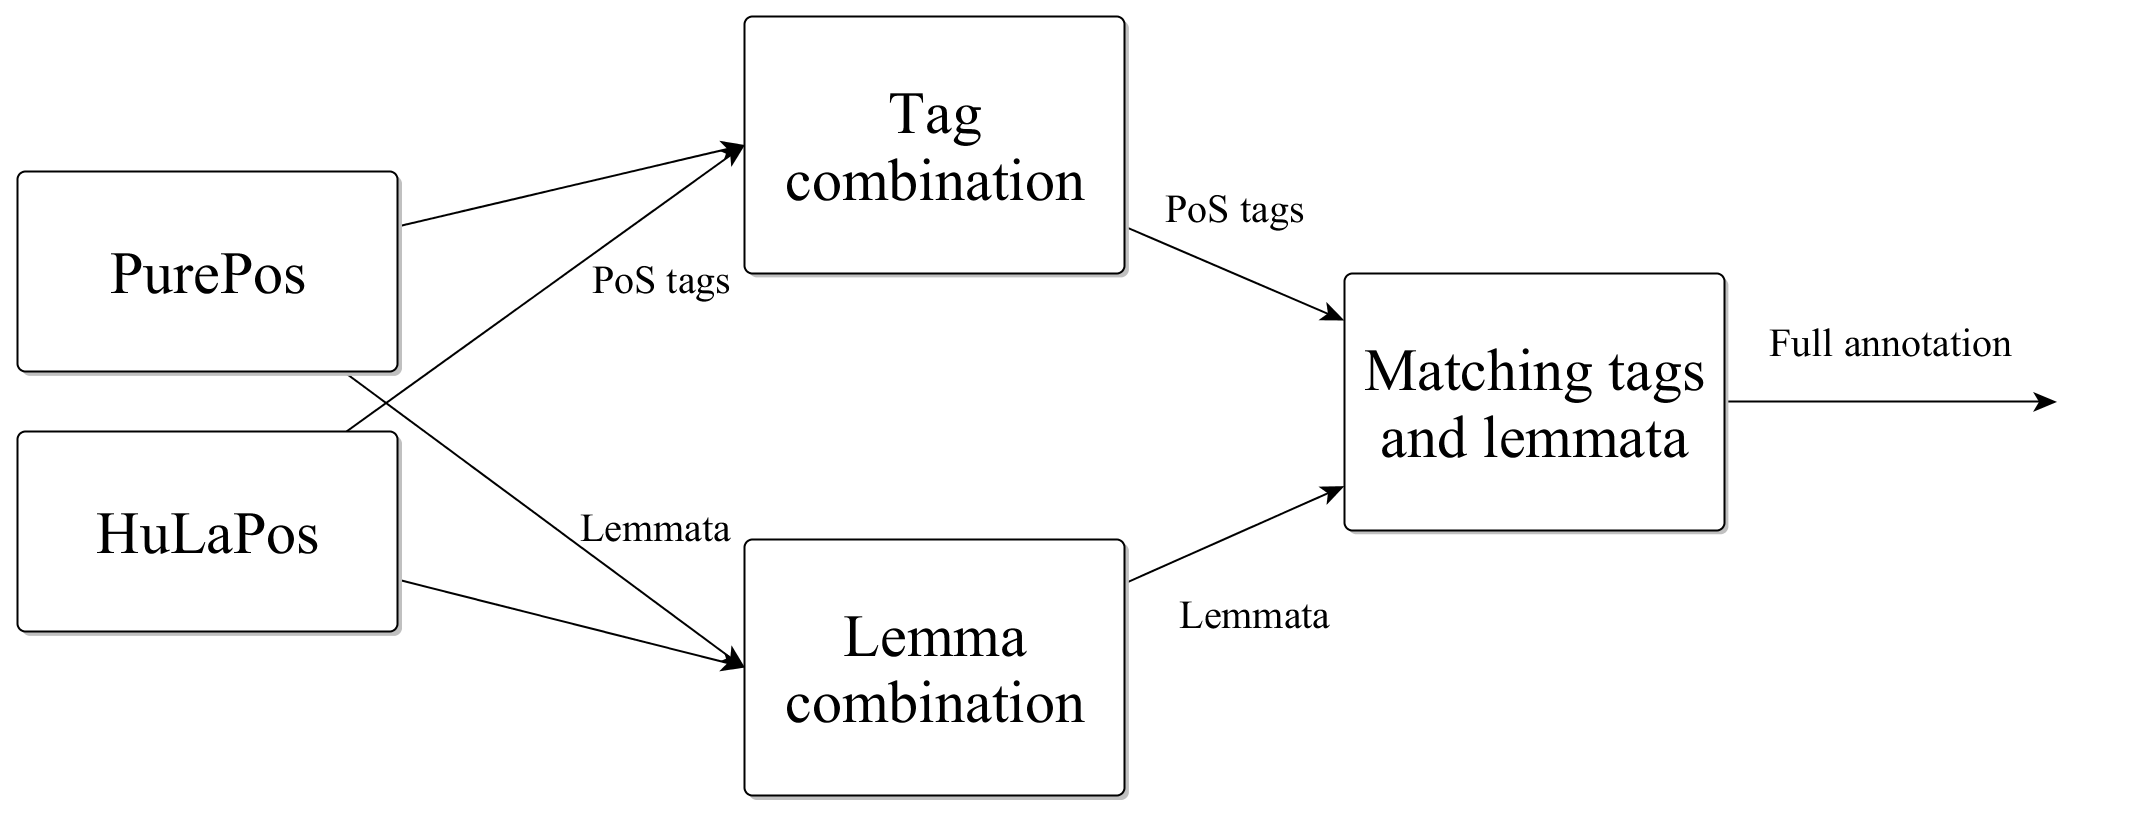
\includegraphics[scale=0.15]{MorphTagging/comb3.png} 
  \caption{Combining the output of two PoS taggers and lemmatizers}
  \label{fig:comb3_en}
\end{figure}

Finally, evaluation experiments were presented indicating that the number errors of the best tagger can be decreased further.
The new algorithm could reduce the number of errors of PurePos by 28.90\%.

\subsection{Measuring morpho-syntactic complexity using morphological annotation algorithms}
\label{thes:mlu}


Measuring morpho-syntactic complexity is usually carried out calculating \acrlong{mlu}s.
This metric is often computed in words for analytical languages, while morphemes (\acrshort{mlum}) are used for morphologically complex ones.
Although automatic methods and tools exist for e.g English, other less-resourced languages lack such systems.
Therefore, \acrshort{mlum} could be only computed manually, which is a time-consuming task.

This thesis group presents\footnote{This research has been conducted together with Kinga Jelencsik-Mátyus. 
%Manual annotation of the data were performed by both of us, while the morpheme counting principles are her work. 
My contributions are the construction of the tagging chain, its adaptation and the automatization of the MLUm calculation.} methods for processing speech transcripts effectively and estimating \acrlong{mlum} automatically.
%Our solution relies on the PurePos tagger tool (cf. Thesis \ref{thes:morf-tagging}).
%Results also indicate that the labor-intense manual work can be replaced with our new method.


\begin{core}
\begin{thesis}
\label{thes:spoken-morf-tagging}
I developed a hybrid morphological tagging chain for Hungarian child-language transcripts.
My method builds on top of the results presented in Thesis \ref{thes:morf-tagging} by adapting them to the domain.
Evaluation shows that performance of the method is comparable with that of tagging methods for written corpora.
Moreover, experiments indicate that the algorithm presented is accurate enough to be used in further applications.
\end{thesis}

\begin{pub}
\cite{Matyus2014,Orosz2014c}
\end{pub}
\end{core}

The proposed method adapts the algorithms introduced in Thesis \ref{thes:morf-tagging} for spoken Hungarian.
For this, the Humor \acrlong{ma} was augmented first with analyses of words typical to the domain.
Next, the output of PurePos was adjusted utilizing domain-specific knowledge.

For this, a gold corpus of about 1,000 utterances from the \acrshort{hukilc} was created by the manual annotation of texts. 
Additionally, a new tagging scheme was designed representing the characteristics of spoken language properly.
%These manually corrected texts enabled us to develop and validate the proposed methods.

The evaluation of the chain resulted in 96\% token-level precision, which is comparable with that of taggers for corpora of written language.
Therefore, my investigation showed that PurePos is an appropriate base for tagging corpora of transcribed spoken texts.

\thesisline%%%%%%%%%%%%%%%%%%%%%%%%%%%%%%%%%%%%%%%%%%%%%%%%%%%%%%%%%%%%%%%%%%%%%


\begin{core}
\begin{thesis}
\label{thes:mlu-estimation}
I proposed a new algorithm for estimating morpho-syntactic complexity (calculating \acrlong{mlum}) in Hungarian child language transcripts.
The method uses the morphological tagging chain of Thesis \ref{thes:spoken-morf-tagging} as a base.
%In doing so, it computes lengths of utterances in its output.
Evaluation of the system indicates that my methodology can properly replace the time-consuming manual computation of human annotators.
\end{thesis}

\begin{pub}
\cite{Matyus2014,Orosz2014c}
\end{pub}
\end{core}

The estimation method analyzes morphological annotations of tokens.
Words known by the analyzer are decomposed by Humor, while lengths of unknown words are guessed based on their \acrshort{pos} labels.
This is followed by morpheme counting rules implementing linguistic guidelines, thus providing relevant estimates.

As regards resources, a manually checked corpus was created for the experiments.
Evaluation of the methods on this dataset shows that my results highly correlate (0.9901) with counts of human annotators.
Further on, I showed that the mean relative error of the method is only 4.49\%.
Thus, the proposed algorithm can properly replace the labor-intensive human computation.

\subsection{Effective preprocessing methods for a less-resourced noisy domain}
\label{thes:clin}

More and more electronic health records are produced in hospitals containing valuable but hidden knowledge.
Since doctors cannot spend enough time on writing their reports properly, notes often contain numerous errors.
Because of such mistakes, processing of such texts cannot be carried out using general-purpose tools.
Moreover, while several algorithms are becoming available for English, Hungarian and other morphologically rich languages are still neglected.

\begin{core}
\begin{thesis}%{II.1/b}
\label{thes:clin-segment}
I developed a new framework which segments noisy clinical records into words and sentences accurately.
The method is built on top of well-known tokenization rules (e.g. \cite{Halacsy2004}), however, it augments them with unsupervised heuristics.
Evaluations showed that the tool can properly identify word and sentence boundaries in noisy clinical notes. 
Results also indicate that other systems available cannot handle such erroneous texts.
\end{thesis}

\begin{pub}
\cite{Orosz2013d,Orosz2014a,Orosz2014x}
\end{pub}
\end{core}

\begin{figure}[H]
  \centering
  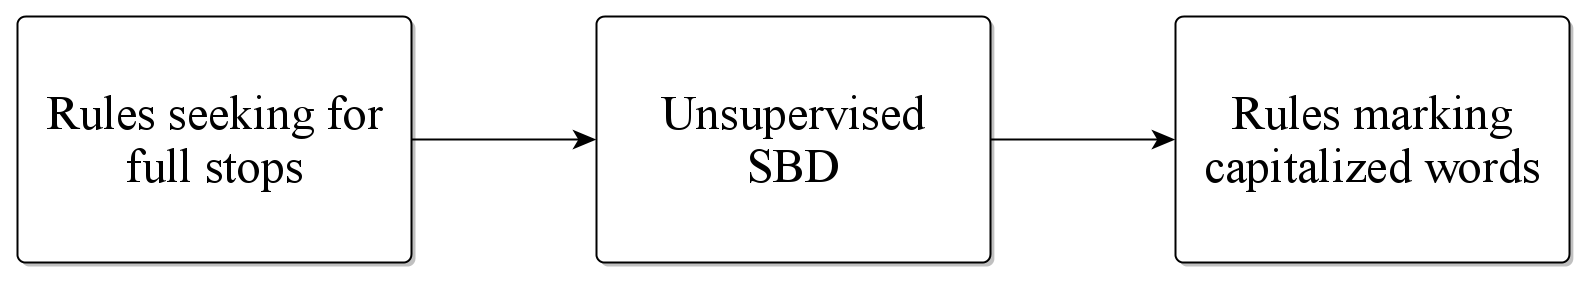
\includegraphics[scale=0.2]{Clinical/clin_segm_arch.png} 
  \caption{The architecture of the proposed method}
  \label{fig:clin-segment-arch_en}
\end{figure}

The proposed method builds on pattern-matching algorithms taken from general-purpose tokenization tools.
Even though these methods perform with high accuracy, their recall still stays low.
Therefore, this study proposes a method (see Figure \ref{fig:clin-segment-arch_en}) which improves their performance using unsupervised heuristics and a domain-specific morphologic analyzer.
First, the scaled $\log\lambda$  method \cite{kiss2006unsupervised} was adapted by introducing new factors.
Next, the Humor morphological analyzer was utilized to reveal further sentence boundaries.

The evaluation of the framework was carried out on a manually segmented corpus. 
Numerous metrics (such as precision, recall, F-score) were employed measuring the performance of the proposed tool.
%Thus, I could analyze both the tokenization and the sentence boundary detection accuracy of the tool.
Moreover, existing Hungarian approaches were also compared with the proposed one.

Results show other available systems can only produce low quality segmentation.
Most of them result in F-scores less than 50\% in sentence boundary identification.
On the contrary, the method proposed can detect both token and sentence boundaries accurately, producing F-values over 90\%.


%%%%%%%%%%%%%%%%%%%%%%%
\thesisline%%%%%%%%%%%%
%%%%%%%%%%%%%%%%%%%%%%%

\begin{core}
\begin{thesis}%{II.2}
\label{thes:clin-pos}
I showed that tagging methods of Thesis \ref{thes:morf-tagging} can be applied for annotating electronic health records satisfactorily.
In doing so, PurePos was adjusted with stochastic and symbolic domain adaptation techniques.
The quality of the annotation produced is comparable with that of general written tagger tools.
\end{thesis}

\begin{pub}
\cite{Orosz2013,Orosz2014b,Orosz2014x} 
\end{pub}
\end{core}

First of all, an extended version of the Humor analyzer was used as a base of the tagging chain, since it was prepared\footnote{The lexicon extension was carried out by Attila Novák \cite{Orosz2014} .} for electronic health records.
Further on, the tagging chain was improved using a detailed error analysis of the baseline tagger.

For this, a manually annotated corpus was created containing texts of clinical notes.
Results on this dataset show that the improved system performs significantly better (93.73\%) than the baseline system (88.09\%).
However, future work might target the segmentation and tagging tasks with a unified framework, since both systems have the most problems with abbreviated terms.

\let\thesubsection=\oldthesubsection